% Compile with XeLaTeX:  latexmk -xelatex main.tex
\documentclass[11pt]{article}
\usepackage[preprint]{acl}
\usepackage{fontspec}
\setmainfont{TeX Gyre Termes}
\newfontfamily\ethiopicfont{AbyssinicaSIL-Regular.ttf}[Path=./, Scale=MatchLowercase, BoldFont=AbyssinicaSIL-Regular.ttf, BoldFeatures={FakeBold=2}]
\newcommand{\am}[1]{{\ethiopicfont #1}}
\usepackage{microtype}
\usepackage{graphicx}
\usepackage{booktabs}
\usepackage{adjustbox}

\title{Amharic Sentiment Analysis Using Ethiopic Character Normalization\\and Multilingual Transformer Fine-tuning}

\author{Eyob Nebyou \\
  Department of Computer Science, College of Natural and Computational Sciences \\
  Addis Ababa University, Addis Ababa, Ethiopia \\
  \texttt{eyobnebyou10@gmail.com}}

\begin{document}
\maketitle
\begin{abstract}
Amharic, a federal working language of Ethiopia with about 57 million first- and second-language speakers, remains severely underrepresented in natural language processing research. In this paper, we present a systematic study of sentiment analysis on Amharic Twitter data using the AfriSenti benchmark. We make three contributions: (1) a structured Ethiopic character normalization pipeline that unifies orthographically equivalent character families and improves the TF-IDF baseline's test macro F1 by 1.7 points in an ablation; (2) a comparison of a TF-IDF and Logistic Regression baseline against fine-tuned Afro-XLM-R, a multilingual transformer pre-trained on 17 African languages; and (3) a native-speaker qualitative error analysis of the baseline and the transformer, identifying five linguistically grounded failure patterns. Our fine-tuned model achieves a macro F1 of \textbf{0.5543 $\pm$ 0.0068} across three random seeds, a \textbf{+9.03 point improvement} over the TF-IDF baseline (0.4640). The error analysis separates three patterns on which the baseline fails and the transformer succeeds (journalistic framing with embedded sentiment words, Amharic negation, and culturally loaded religious language) from two on which both models fail (news-framed atrocity reporting and Amharic praise song structure); a feature analysis additionally shows the baseline learning a political name as a strong negative cue.

\end{abstract}


\section{Introduction}

Sentiment analysis --- the automatic classification of text as positive, negative, or neutral --- is one of the most widely deployed NLP tasks, with applications ranging from brand monitoring and public health surveillance to content moderation and political analysis. Despite this broad utility, the vast majority of sentiment analysis systems are built for high-resource languages such as English, Chinese, and Arabic. Amharic is spoken by about 57 million people, 31.8 million as a first language and 25.1 million as a second language \citep{eberhard-etal-2020-ethnologue}, and is a federal working language of Ethiopia. Yet it has far fewer sentiment resources and tools than languages of comparable size.

This gap matters in practice. Without reliable Amharic sentiment models, institutions and media organizations in Ethiopia have limited means to analyze public opinion expressed in Amharic at scale, and researchers studying Ethiopian online discourse must rely largely on manual annotation.

This paper addresses that gap through three contributions:

\begin{enumerate}
\def\labelenumi{\arabic{enumi}.}
\item
  \textbf{Ethiopic normalization}: We introduce and evaluate a character normalization pipeline that unifies orthographically equivalent Ethiopic characters (e.g., the ha-family variants \am{ሀ/ሐ/ኀ}, and the sa-family variants \am{ሠ/ሰ}), applied before both classical and neural modeling. An ablation on the TF-IDF baseline shows that it reduces the number of unigram types by 2.5\% and improves test macro F1 by 1.7 points.
\item
  \textbf{Systematic comparison}: We compare a TF-IDF + Logistic Regression baseline against Afro-XLM-R fine-tuned on the AfriSenti Amharic sentiment dataset, reporting results across three random seeds for statistical reliability.
\item
  \textbf{Native speaker error analysis}: As a native Amharic speaker, the author conducts a qualitative analysis of model failures, identifying five failure patterns that aggregate metrics alone do not reveal: three that the baseline exhibits and the transformer corrects (journalistic syntax with embedded sentiment words, negation blindness, and culturally loaded positive religious language) and two that both systems share (news-framed atrocity reporting and Amharic praise song structure). We additionally report a political entity bias in the baseline's learned features. These patterns were identified through close reading of examples by a native speaker.
\end{enumerate}

Our results show that fine-tuned Afro-XLM-R achieves a macro F1 of 0.5543 $\pm$ 0.0068, representing a 19.5\% relative improvement over the TF-IDF baseline. We further identify that a severe train/test distribution shift --- the test set is 66.9\% negative versus 25.9\% negative in training --- constitutes a systematic challenge for all evaluated systems.


\section{Related Work}

\textbf{AfriSenti and African NLP.} \citet{muhammad-etal-2023-afrisenti} introduced AfriSenti, a Twitter sentiment benchmark covering 14 African languages, which formed the basis of the SemEval-2023 Task 12 shared task \citep{muhammad-etal-2023-semeval}. The Amharic subset, which we use in this work, contains 9,480 tweets across train, validation, and test splits. The shared task was evaluated with weighted F1, and its monolingual track (Task A) was won on average by NLNDE. On Amharic, the organizers' baseline, a fine-tuned AfroXLMR-large, scored 61.60 weighted F1, and the best system, GMNLP, scored 78.42 using phylogeny-based adapter tuning of AfroXLMR-large with dictionary- and machine-translation-based data augmentation. Because we report macro F1 and fine-tune only a base-size model, our results are not directly comparable to these figures. We position our work as a reproducible, methodologically transparent baseline that contributes native-speaker analysis rather than ensemble or adaptation complexity.

\textbf{Multilingual and African language models.} \citet{conneau-etal-2020-unsupervised} introduced XLM-RoBERTa (XLM-R), a cross-lingual transformer trained on 2.5 terabytes of CommonCrawl data across 100 languages. \citet{alabi-etal-2022-adapting} extended this work to produce Afro-XLM-R, continuing pre-training on text from 17 African languages including Amharic. This Africa-aware checkpoint is the foundation of our fine-tuned model. \citet{ogueji-etal-2021-small} showed that a model pre-trained only on African languages can be competitive with large multilingual models on African-language tasks, and \citet{alabi-etal-2022-adapting} found that their adapted model outperformed XLM-R on most of the African languages they evaluated, which motivates our choice of Afro-XLM-R over vanilla XLM-R.

\textbf{Amharic NLP.} Amharic NLP research has grown in recent years. \citet{belay-etal-2021-impacts} studied the impact of Ethiopic homophone normalization on Amharic semantic models and found that its effect depends on the application: it was essential for information retrieval but had negative impacts on sentiment analysis and part-of-speech tagging. \citet{belay-etal-2022-effect} later found that normalization improves Amharic--English machine translation, while \citet{nigatu-etal-2025-case} argue that normalizing homophones amounts to an implicit standard and may affect how well models handle varied writing and transfer across languages. Our ablation (Section 5.1) tests normalization directly for sentiment classification, where the earlier result was negative, and finds a modest gain for a TF-IDF baseline. We do not test its effect on the transformer. \citet{tonja-etal-2024-ethiollm} evaluated several multilingual and Ethiopia-specific language models on Amharic sentiment using AfriSenti, reporting F1 scores of approximately 61\% for XLM-R-large, AfroLM-large, and EthioLLM-large and 58\% for EthioLLM-base, which illustrates the difficulty of the task. Differences in evaluation setup and F1 averaging may limit direct comparison with our macro F1. Deep learning approaches on smaller, domain-specific datasets have reported higher accuracy figures (e.g., 91.60\% for a hybrid CNN--BiLSTM on Amharic political comments, in a binary-label setting \citep{alemayehu-etal-2023-amharic}), but these are not directly comparable due to differences in data and task.


\section{Dataset}

We use the AfriSenti Amharic subset (\texttt{masakhane/afrisenti}, config \texttt{amh}) available through the HuggingFace Datasets library. The dataset consists of tweets collected from Ethiopian Twitter and manually annotated for sentiment.

\textbf{Dataset statistics.} Table~\ref{tab:data} gives the label counts for each split.

\begin{table}[t]
\centering\small
\begin{adjustbox}{max width=\linewidth}
\begin{tabular}{lrrrr}
\toprule
Split & Samples & Negative & Neutral & Positive \\
\midrule
Train & 5,984 & 1,548 (25.9\%) & 3,104 (51.9\%) & 1,332 (22.3\%) \\
Validation & 1,497 & 388 (25.9\%) & 776 (51.8\%) & 333 (22.2\%) \\
Test & 1,999 & 1,337 (66.9\%) & 224 (11.2\%) & 438 (21.9\%) \\
\bottomrule
\end{tabular}
\end{adjustbox}
\caption{AfriSenti Amharic label counts per split, before preprocessing.}
\label{tab:data}
\end{table}

\textbf{Distribution shift.} A critical finding from our data analysis is a severe label distribution shift between training and test splits. The training set is dominated by neutral tweets (51.9\%), while the test set is dominated by negative tweets (66.9\%). The validation split, by contrast, matches the training distribution almost exactly. This shift is not an artifact of our preprocessing --- it is present in the original dataset release. This shift creates a systematic challenge: models trained to predict the most frequent training label (neutral) are evaluated on a test set where that label is the minority class. We report this finding explicitly because it partially explains the gap between absolute performance figures and the perceived difficulty of the task. Figure 1 shows the shift.

\begin{figure}[t]
\centering
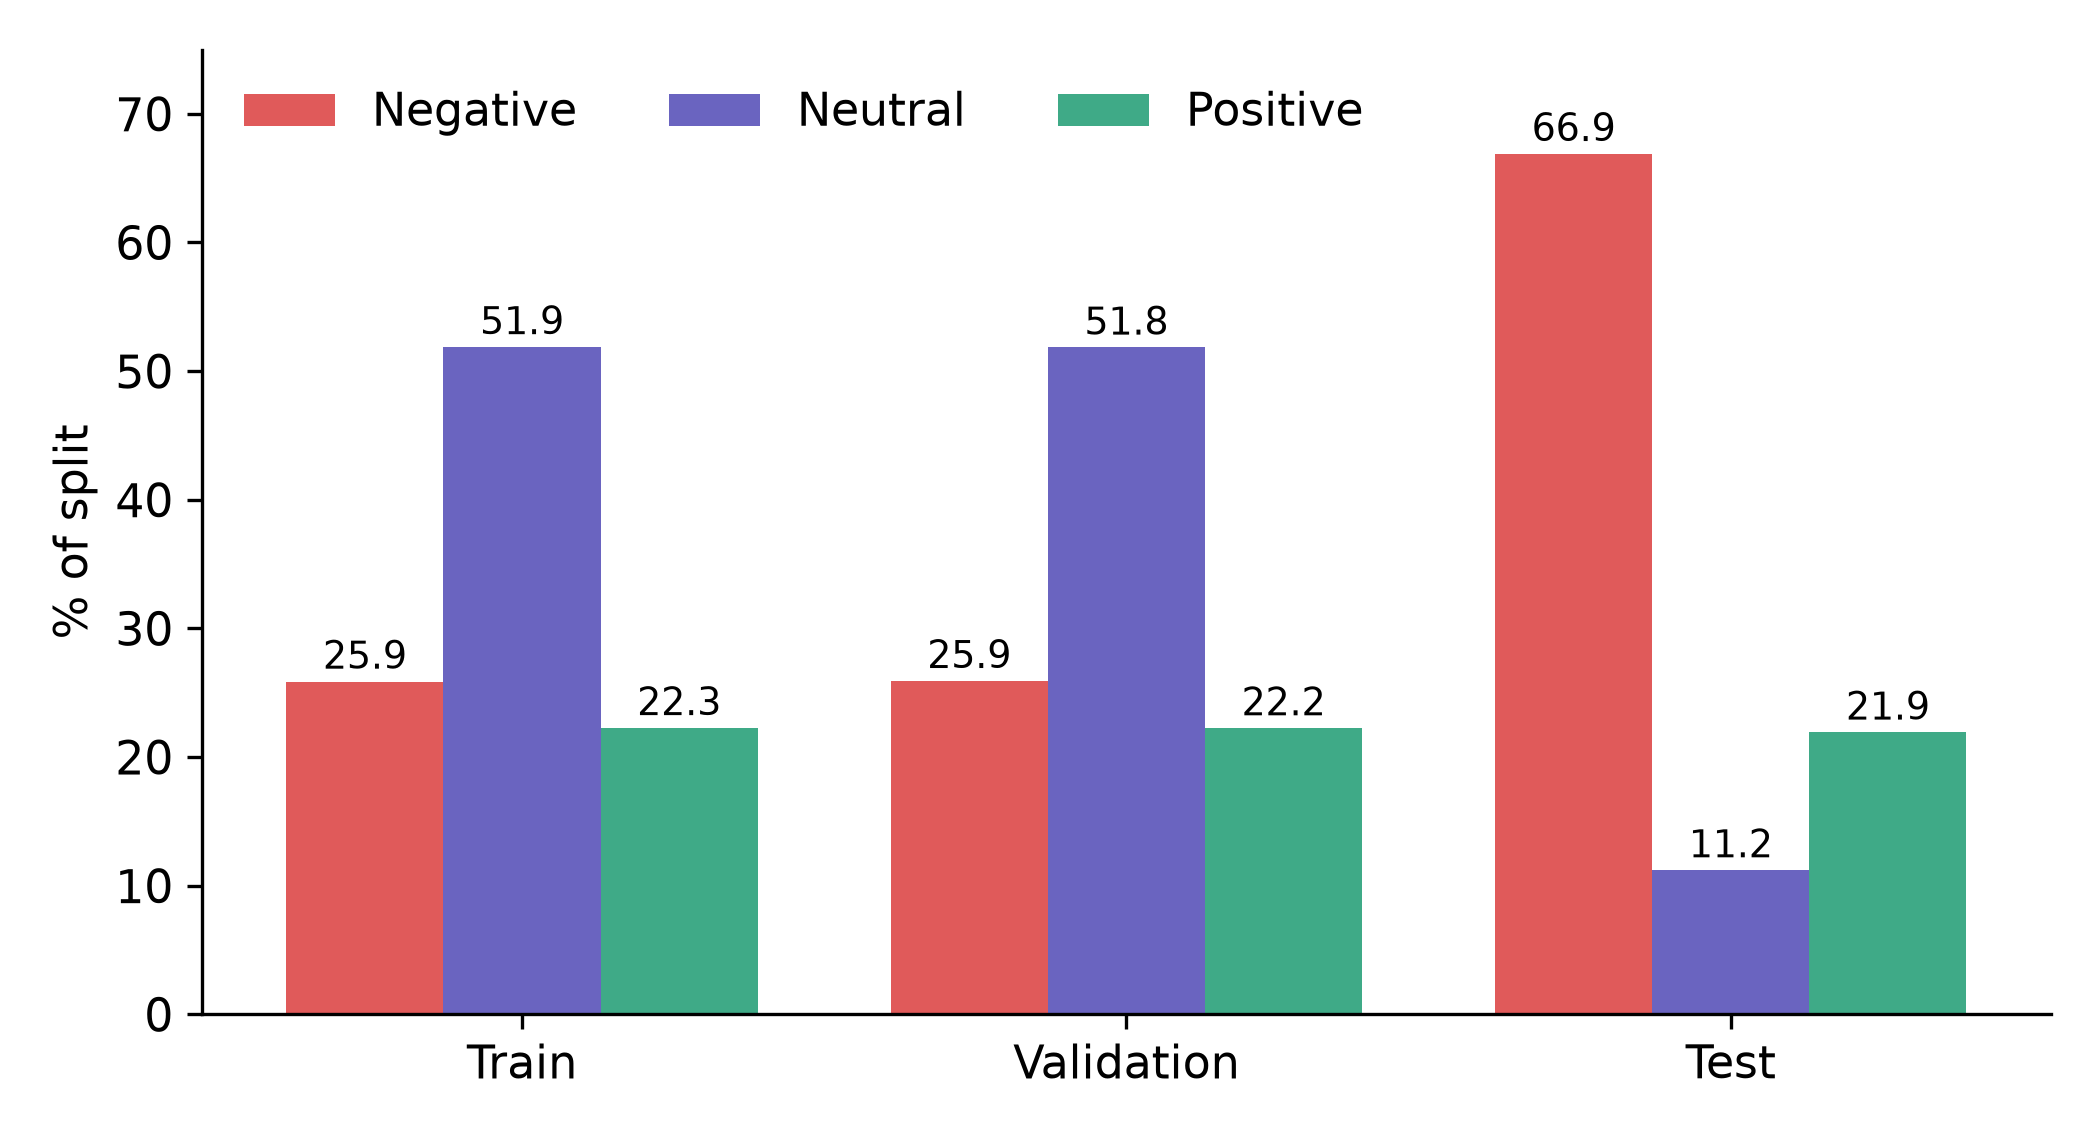
\includegraphics[width=\columnwidth]{figures/paper_fig1_label_shift.png}
\caption{Label distribution (\% of tweets) in each split of the AfriSenti Amharic data. Validation matches training; the test split is dominated by negative tweets and has few neutral ones.}
\label{fig:shift}
\end{figure}
\textbf{Additional data quality findings.} Manual inspection of the dataset by the author, a native Amharic speaker, revealed two additional quality issues: (1) label noise, both in the neutral class, where several tweets expressing clear positive or negative sentiment are labeled neutral, and in the positive class, where polite constructive suggestions --- which we judge to be neutral --- are sometimes labeled positive (e.g., \am{ምንጭ ዲ/ን ዳንኤል ክብረት ብለው ቢጠቅሱ ጥሩ ነበር}, ``it would have been better to cite Daniel Kibret as the source''); and (2) the presence of Tigrinya tweets --- Tigrinya shares the Ethiopic script with Amharic but is a distinct language --- which introduces cross-lingual noise. We did not filter or count these tweets: because the two languages share a script, rule-based filtering without a dedicated language-identification model cannot cleanly separate them, so they remain in all splits. Both issues are characteristic of social media data collected at scale and reflect real-world conditions for which deployed systems must be robust.

\textbf{Text characteristics.} Average tweet length is 14.42 words (std: 7.09). Mixed-script tweets (containing both Ethiopic and Latin characters) constitute 10.4\% of the training set, primarily due to English code-switching and proper nouns. The training and validation splits contain no @mentions or hashtags (and the training split contains no URLs), but the test split does: 1,245 of 1,999 test tweets (62.3\%) contain an @user mention and 101 (5.1\%) contain a hashtag. This format difference is a further train/test mismatch beyond the label shift, and it is why noise removal (Section 4.1) matters.


\section{Methodology}

\subsection{Preprocessing Pipeline}

We apply a five-step preprocessing pipeline to all splits before modeling:

\textbf{Step 1: Noise removal.} We remove URLs, @mentions, and hashtags using regular expressions. This step is necessary: although the training and validation splits contain none of these elements, 62.3\% of test tweets contain an @user mention and 5.1\% a hashtag (Section 3).

\textbf{Step 2: Ethiopic character normalization.} Amharic orthography includes several families of visually and phonetically similar characters that are used interchangeably in informal writing. For example, the characters \am{ሀ}, \am{ሐ}, and \am{ኀ} all represent similar sounds in contemporary Amharic usage but are treated as distinct vocabulary items by bag-of-words models. We normalize these to canonical forms across four character families: the ha-family (\am{ሀ/ሐ/ኀ}), the sa-family (\am{ሠ/ሰ}), the glottal a-family (\am{አ/ዓ}), and the tsa-family (\am{ፀ/ጸ}). The mapping covers all seven vowel orders of the \am{ሐ}-, \am{ኀ}-, \am{ሠ}-, and \am{ፀ}-families (e.g., \am{ሑ}$\rightarrow$\am{ሁ}, \am{ሡ}$\rightarrow$\am{ሱ}), together with the labialized forms \am{ሗ} and \am{ሧ}. For the glottal a-family, the second, third, and fifth to seventh orders of \am{ዐ} map to the corresponding orders of \am{አ} (e.g., \am{ዑ}$\rightarrow$\am{ኡ}), while \am{ዓ} and \am{ኣ} (fourth order) both map to the first-order \am{አ}; the first-order \am{ዐ} itself is not mapped. The effect of this step on the TF-IDF baseline is evaluated in Section 5.1.

\textbf{Step 3: Special character removal.} We retain Ethiopic script (Unicode range U+1200--U+137F), Latin characters, digits, and Ethiopic punctuation marks (\am{።}, \am{፣}). All other characters, including emojis and non-standard punctuation, are removed.

\textbf{Step 4: Latin lowercasing.} Latin characters, which appear in code-switched tokens and proper nouns, are lowercased for consistency. Ethiopic characters are case-invariant and are left unchanged.

\textbf{Step 5: Short-text check and deduplication.} 48 training tweets (0.8\%) contain fewer than two words; we count but retain them. After cleaning, tweets whose cleaned text is empty or identical to an earlier tweet in the same split are removed (16 training rows, 1 validation row, 0 test rows). Deduplication is applied within each split. We also checked for overlap across splits (exact matches on the cleaned text, and near-duplicates with cosine similarity of at least 0.9 on binary word vectors). At most two test tweets (0.1\%) have an exact or near-duplicate in the training set, and none overlap with validation. Validation overlaps with training more: 5 tweets (0.3\%) match a training tweet exactly after cleaning, and 52 (3.5\%) have a non-identical near-duplicate in training. We leave all of these in place.

After preprocessing, the training set contains 5,968 tweets, validation 1,496, and test 1,999.

\subsection{TF-IDF Baseline}

We construct a TF-IDF baseline using unigrams and bigrams, a vocabulary ceiling of 50,000 features, a minimum document frequency of 2, and sublinear TF scaling; the resulting vocabulary contains 13,791 features, so the ceiling is never reached. After fitting on the training set, we evaluate three classifiers with fixed, untuned hyperparameters: Linear SVM (C = 1.0), Logistic Regression (C = 1.0), and Random Forest (200 trees, maximum depth 20), all with balanced class weights to counter the label imbalance in the training set. The TF-IDF vectorizer is fitted exclusively on training data to prevent test set leakage. We select the best-performing classifier on the validation set for reporting.

\subsection{Transformer Fine-tuning}

We fine-tune \texttt{Davlan/afro-xlmr-base} --- the base variant of Afro-XLM-R, containing approximately 278 million parameters --- using the HuggingFace Trainer API. We choose the base model over the large variant for computational accessibility on a single T4 GPU.

\textbf{Tokenization.} We use the SentencePiece tokenizer associated with Afro-XLM-R, a unigram language-model tokenizer \citep{kudo-richardson-2018-sentencepiece} inherited from XLM-R, with a vocabulary of 250,002 tokens. We set MAX\_LENGTH = 72 tokens, derived from the 99th percentile of tokenized sequence lengths (67 tokens), rounded up to the nearest multiple of 8 for GPU memory efficiency. This setting truncates only 0.30\% of the dataset.

\textbf{Fragmentation analysis.} The mean fragmentation ratio --- the average number of subword tokens per word --- is 2.220 (std: 0.809) for the training set. This figure is higher than what is typically observed for high-resource languages, confirming that the Afro-XLM-R vocabulary, while Africa-aware, does not provide dense coverage of all Ethiopic morphological forms. Per-class means are nearly identical (negative 2.246, neutral 2.187, positive 2.269). The positive class has a much larger standard deviation (1.517 vs.~\textasciitilde0.43 for the other classes), but this is driven by four outlier tweets (0.3\% of the positive class) rather than a class-wide effect: excluding them, the positive-class standard deviation is 0.477. Three of the four use the Ethiopic word separator character \am{፡} in place of spaces, which joins multiple words into a single whitespace-delimited unit and inflates the subwords-per-word ratio, and one uses character repetition for emphasis (e.g., \am{እልልልልልልልልልልልል}), which produces extreme out-of-vocabulary fragmentation.

\textbf{Training configuration.} We use the following hyperparameters: learning rate $2\times10^{-5}$, batch size 32, up to 5 epochs with early stopping (patience: 2 epochs based on validation macro F1), and weight decay 0.01 with 100 warm-up steps. Mixed-precision training (fp16) is enabled. The loss is standard unweighted cross-entropy, whereas the baseline classifiers use balanced class weights. We report results across three random seeds (42, 123, 456) to assess stability.


\section{Experiments and Results}

\subsection{Baseline Results}

\begin{table}[t]
\centering\small
\begin{adjustbox}{max width=\linewidth}
\begin{tabular}{lccc}
\toprule
Model & Val F1 & Test F1 & Test Acc. \\
\midrule
Linear SVM & 0.4972 & 0.4139 & 0.4277 \\
Random Forest & 0.4975 & 0.4099 & 0.4202 \\
Logistic Regression & \textbf{0.5256} & \textbf{0.4640} & \textbf{0.4997} \\
\bottomrule
\end{tabular}
\end{adjustbox}
\caption{TF-IDF baselines (macro F1 and accuracy).}
\label{tab:baselines}
\end{table}

Logistic Regression outperforms the Linear SVM on both validation (0.5256 vs.~0.4972) and test (0.4640 vs.~0.4139) macro F1. Because the validation split shares the training distribution, this advantage cannot be attributed to the train/test label shift. We did not tune hyperparameters for any classifier, so we make no claim about its cause.

\textbf{Normalization ablation.} To isolate the effect of Ethiopic normalization (Step 2), we retrain the Logistic Regression baseline with that step removed, keeping all other preprocessing, features, and hyperparameters unchanged. Both conditions use exactly the same rows.

\begin{table}[t]
\centering\small
\begin{adjustbox}{max width=\linewidth}
\begin{tabular}{lcccc}
\toprule
Preprocessing & Types & Val F1 & Test F1 & Test Acc. \\
\midrule
Without norm. & 31,462 & 0.5199 & 0.4474 & 0.4812 \\
With norm. & 30,679 & 0.5256 & \textbf{0.4640} & \textbf{0.4997} \\
\bottomrule
\end{tabular}
\end{adjustbox}
\caption{Normalization ablation for the Logistic Regression baseline. Types: unigram types in the preprocessed training set. F1 is macro F1.}
\label{tab:ablation}
\end{table}

Unigram types are counted on the training set after preprocessing, with no frequency threshold. Normalization improves test macro F1 by 1.66 points (95\% paired bootstrap CI {[}+0.80, +2.62{]}, resampling test examples) and validation macro F1 by 0.57 points, and it reduces the number of unigram types by 2.5\%. The gain is modest, and the size of the 1--2-gram TF-IDF vocabulary is essentially unchanged (13,793 vs.~13,791 features) because of the minimum document frequency threshold. The bootstrap interval reflects test-set sampling only and does not capture variation from training.

\subsection{Per-class Baseline Performance}

\begin{table}[t]
\centering\small
\begin{adjustbox}{max width=\linewidth}
\begin{tabular}{lcccr}
\toprule
Class & Precision & Recall & F1 & Support \\
\midrule
Negative & 0.84 & 0.48 & 0.61 & 1,337 \\
Neutral & 0.16 & 0.59 & 0.26 & 224 \\
Positive & 0.54 & 0.52 & 0.53 & 438 \\
\bottomrule
\end{tabular}
\end{adjustbox}
\caption{Per-class test performance of the TF-IDF + Logistic Regression baseline.}
\label{tab:baseline-perclass}
\end{table}

The neutral class is by far the hardest --- an F1 of 0.26 reflects both the class's small size in the test set (224 samples) and the fundamental difficulty of distinguishing neutral from mildly positive or mildly negative content.

\subsection{Transformer Results}

\begin{table*}[t]
\centering\small
\begin{adjustbox}{max width=\linewidth}
\begin{tabular}{lcccccc}
\toprule
Seed & Val Macro F1 & Test Macro F1 & Test Weighted F1 & Neg F1 & Neu F1 & Pos F1 \\
\midrule
42 & 0.6027 & 0.5620 & 0.6626 & 0.7337 & 0.3433 & 0.6090 \\
123 & 0.6105 & 0.5553 & 0.6458 & 0.7037 & 0.3330 & 0.6292 \\
456 & 0.5923 & 0.5455 & 0.6294 & 0.6793 & 0.3235 & 0.6337 \\
\midrule
Mean $\pm$ std & 0.6018 $\pm$ 0.0075 & \textbf{0.5543 $\pm$ 0.0068} & 0.6459 $\pm$ 0.0136 & 0.7056 $\pm$ 0.0222 & 0.3333 $\pm$ 0.0081 & 0.6240 $\pm$ 0.0107 \\
\bottomrule
\end{tabular}
\end{adjustbox}
\caption{Fine-tuned Afro-XLM-R base across three seeds. Per-class columns are test F1.}
\label{tab:seeds}
\end{table*}

Validation macro F1 is for the checkpoint selected by early stopping, and all test scores come from that checkpoint. Weighted F1 averages the per-class F1 scores by class support and is the metric used by the SemEval-2023 shared task. Std is the population standard deviation over the three seeds (for test macro F1 the sample standard deviation is 0.0083). Per-class F1 varies more across seeds than macro F1 does, most of all on the negative class (0.679 to 0.734).

\subsection{Comparison}

\begin{table*}[t]
\centering\small
\begin{adjustbox}{max width=\linewidth}
\begin{tabular}{lccccc}
\toprule
System & Macro F1 & Weighted F1 & Neg F1 & Neu F1 & Pos F1 \\
\midrule
TF-IDF + Logistic Regression & 0.4640 & 0.5523 & 0.6107 & 0.2550 & 0.5262 \\
Afro-XLM-R base (mean $\pm$ std, 3 seeds) & \textbf{0.5543 $\pm$ 0.0068} & \textbf{0.6459 $\pm$ 0.0136} & \textbf{0.7056 $\pm$ 0.0222} & \textbf{0.3333 $\pm$ 0.0081} & \textbf{0.6240 $\pm$ 0.0107} \\
\bottomrule
\end{tabular}
\end{adjustbox}
\caption{Test-set comparison of the baseline and the fine-tuned transformer.}
\label{tab:comparison}
\end{table*}

\begin{figure}[t]
\centering
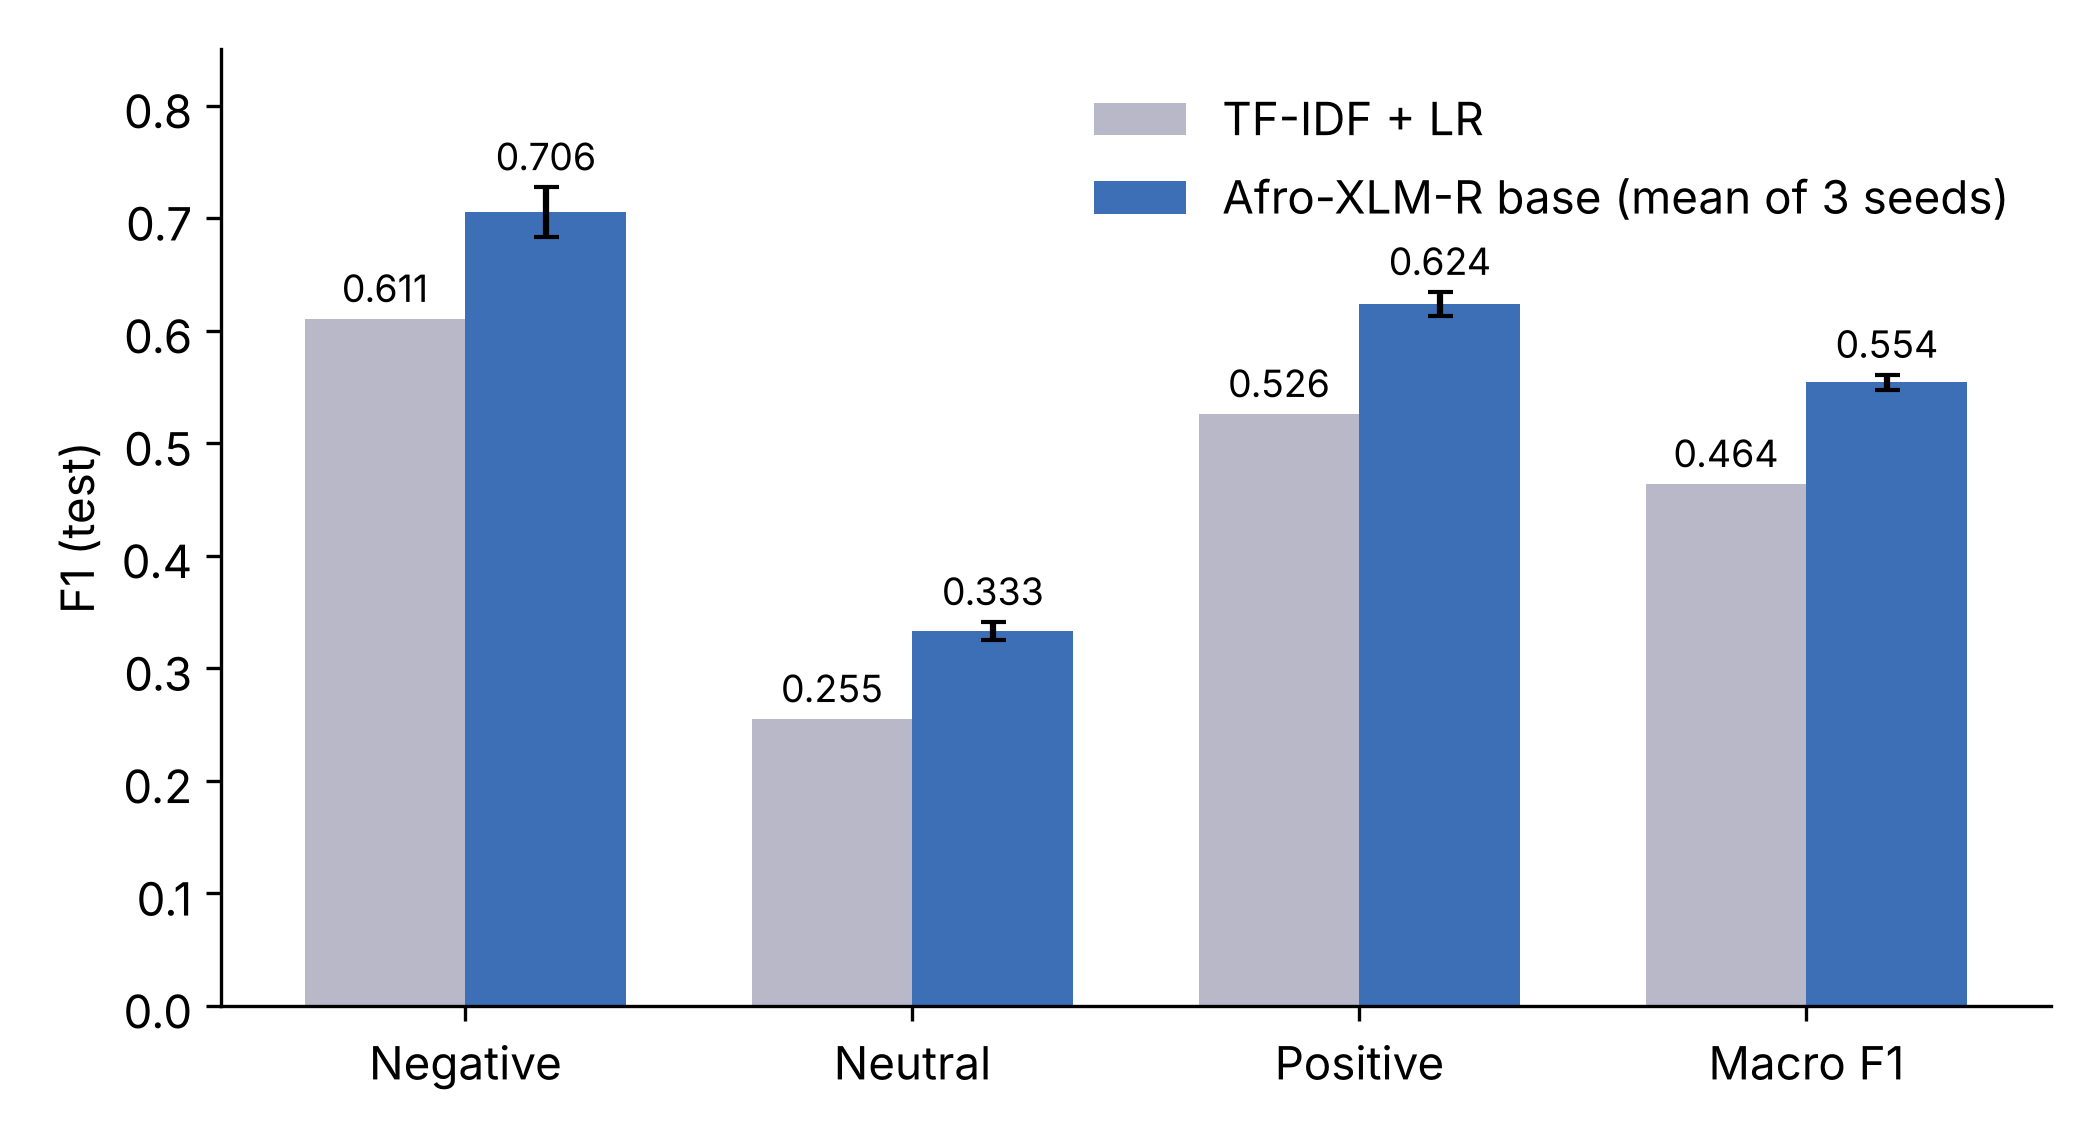
\includegraphics[width=\columnwidth]{figures/paper_fig3_f1.png}
\caption{Test F1 per class and macro F1. Transformer bars show the mean over three seeds, with error bars of one (population) standard deviation.}
\label{fig:f1}
\end{figure}
Averaged over the three seeds (Figure 2), the transformer improves over the baseline on all three classes: by 9.8 F1 points on the positive class, 9.5 on the negative class, and 7.8 on the neutral class, and by 9.4 points in weighted F1. The neutral class remains the hardest for the transformer (mean F1 0.3333), consistent with its small test set size and the label noise identified in our data analysis.

Figure 3 shows where the gain comes from for the seed-42 model. The transformer recovers more negative tweets than the baseline (822 vs.~640 of 1,337), mainly because fewer of them are predicted neutral (446 vs.~532). Its recall on positive tweets is the same as the baseline's (0.52), and its higher positive F1 comes from better precision: it predicts positive for 69 negative tweets against the baseline's 165. Both systems still assign a large share of negative and positive tweets to neutral.

\begin{figure*}[t]
\centering
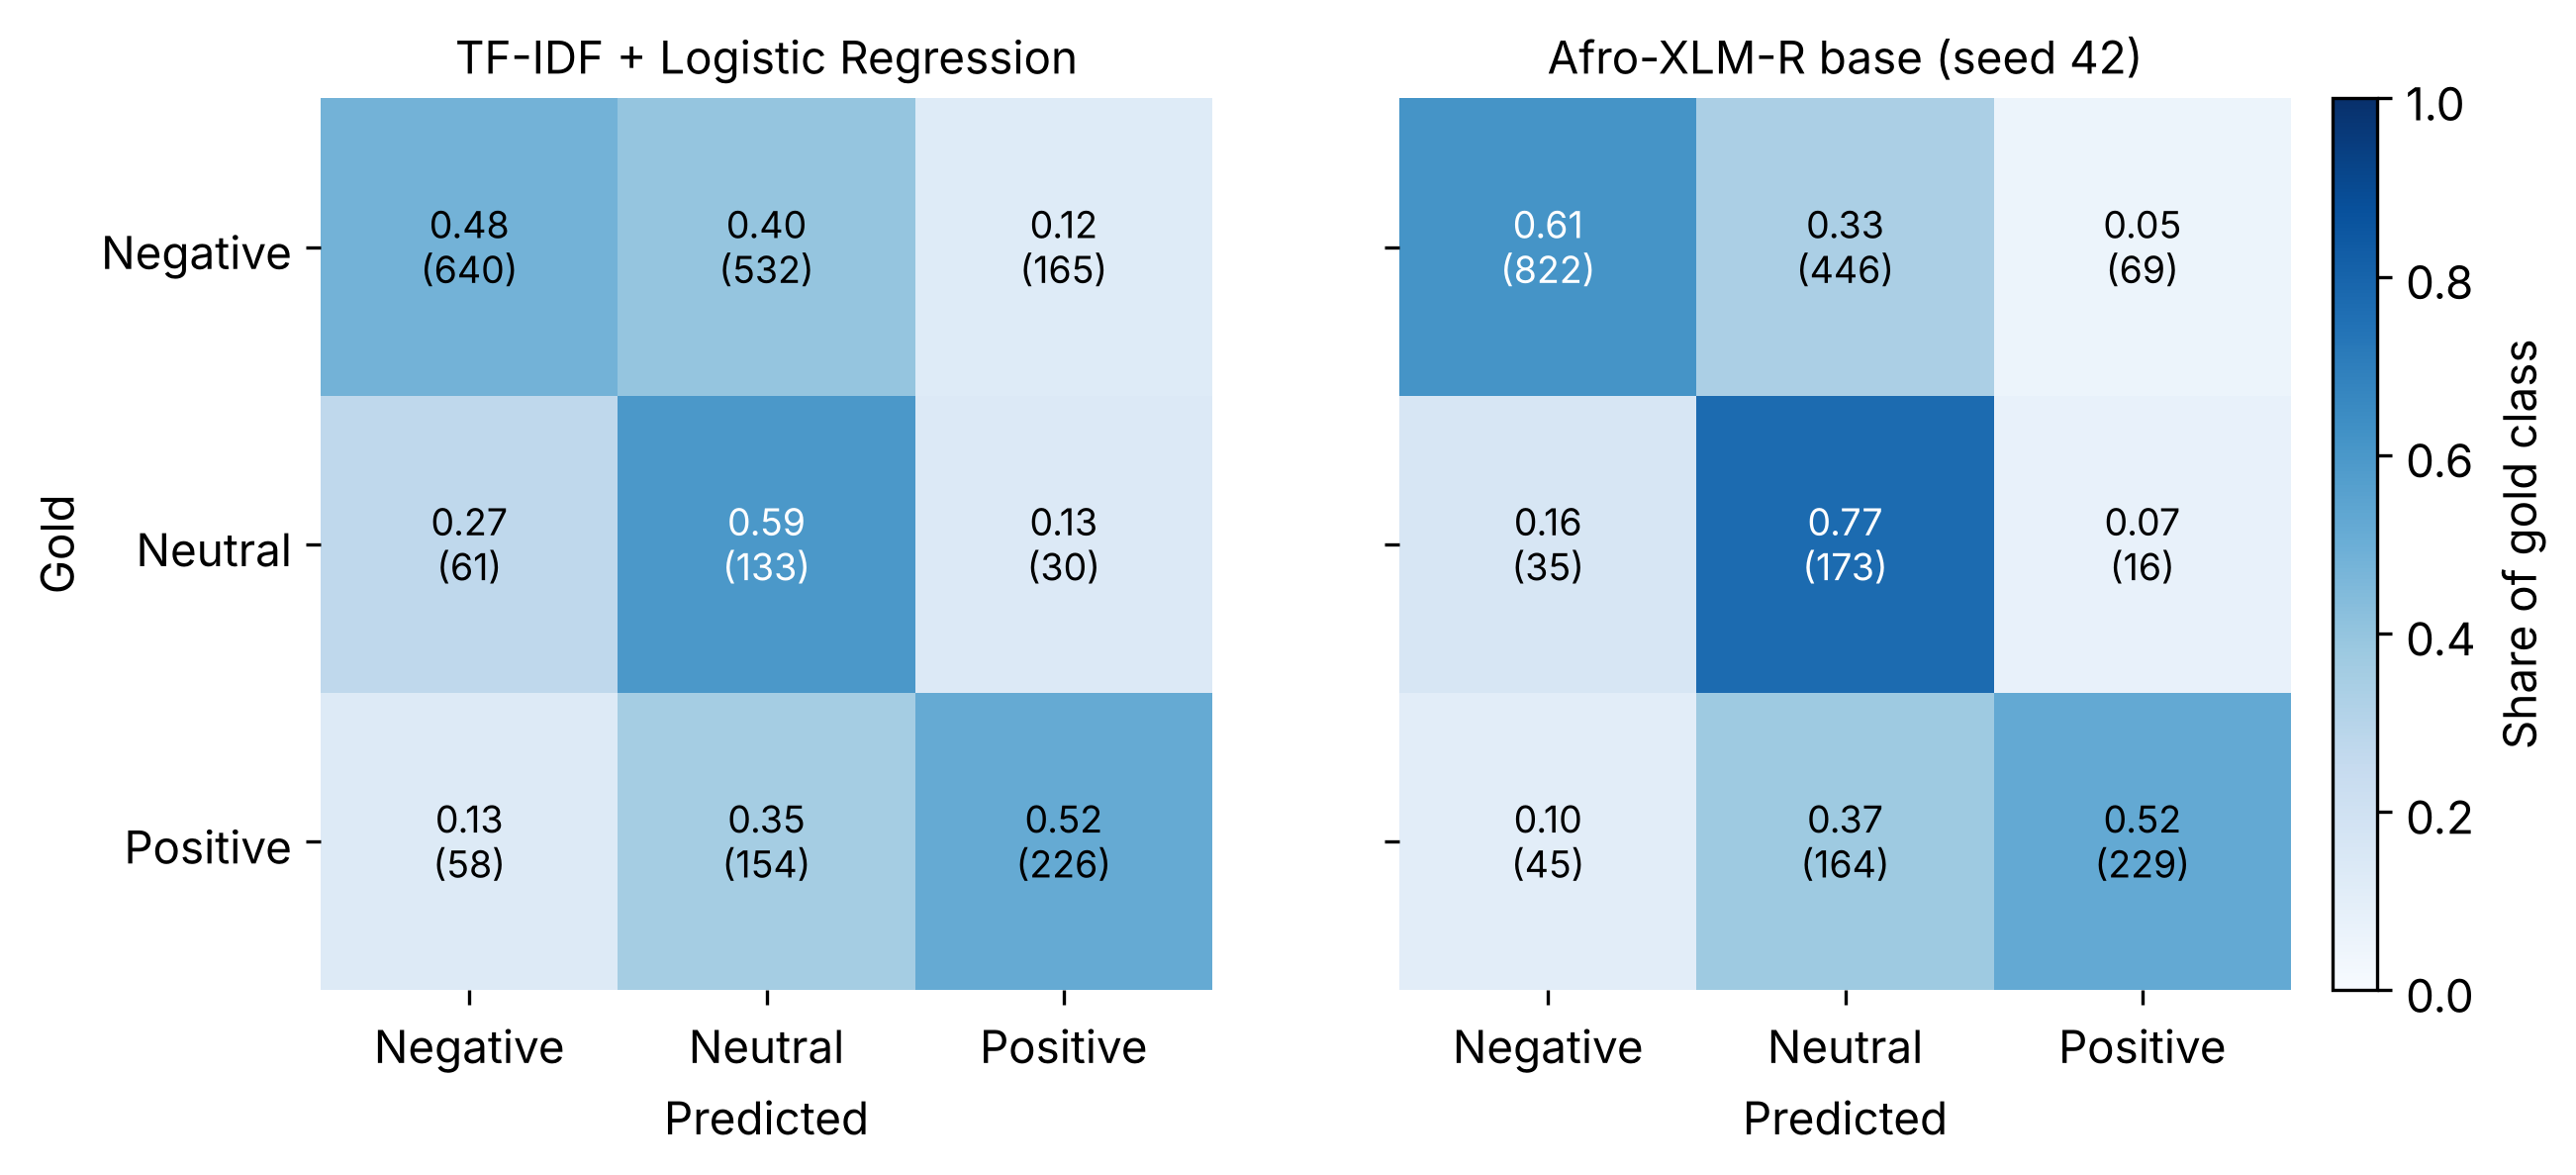
\includegraphics[width=0.8\textwidth]{figures/paper_fig2_confusion.png}
\caption{Confusion matrices on the test set, normalized by gold class (rows), with raw counts in parentheses. Left: TF-IDF + Logistic Regression. Right: Afro-XLM-R base, seed 42 (fp32 inference, as in Section 6).}
\label{fig:confusion}
\end{figure*}
On the shared task's metric, our base-size model's mean weighted F1 (0.6459) is above the organizers' AfroXLMR-large baseline for Amharic (61.60) and below the best submission (78.42) \citep{muhammad-etal-2023-semeval}. These comparisons are indicative only: model size and training procedures differ, and the official test set has 2,000 tweets versus 1,999 here.

The low standard deviation of macro F1 across seeds (0.0068) indicates that the improvement over the baseline is stable and not attributable to a favorable random initialization: all three seeds individually outperform the baseline on both macro and weighted F1.


\section{Error Analysis}

To understand where the transformer adds value and where both systems fail, we categorize all 1,999 test examples into four outcome groups, using the seed-42 transformer. We chose seed 42 because it has the highest test macro F1 of the three seeds. This is a descriptive choice, not model selection, since seed 123 has the highest validation macro F1 (0.6105 vs.~0.6027). The predictions in this section come from fp32 inference of the saved seed-42 checkpoint on CPU, which gives a test macro F1 of 0.5623; the fp16 GPU evaluation used elsewhere in the paper gives 0.5620 for the same checkpoint, a negligible numerical difference. We did not check whether seeds 123 and 456 classify the quoted example tweets identically.

\begin{table}[t]
\centering\small
\begin{adjustbox}{max width=\linewidth}
\begin{tabular}{lrr}
\toprule
Category & Count & \% of test \\
\midrule
Both models correct & 750 & 37.5\% \\
Transformer only correct & 474 & 23.7\% \\
Baseline only correct & 249 & 12.5\% \\
Both models wrong & 526 & 26.3\% \\
\bottomrule
\end{tabular}
\end{adjustbox}
\caption{Test outcomes for the baseline and the seed-42 transformer.}
\label{tab:outcomes}
\end{table}

We organize the patterns we observed by how the two systems behave on them. Section 6.1 covers three patterns on which the baseline fails and the transformer succeeds, Section 6.2 covers two patterns on which both systems fail, and Section 6.3 reports a separate bias observed in the baseline's learned features. The patterns come from the examples we read; we did not annotate every error, so we do not report per-pattern frequencies, and the examples come from one seed's predictions.

\subsection{Where the Transformer Wins}

The transformer correctly classifies 474 tweets (23.7\%) that the baseline fails on. Of these, 349 (73.6\%) are gold-negative, 64 (13.5\%) neutral and 61 (12.9\%) positive; for reference, negative tweets make up 66.9\% of the test set, so the transformer's gains are only mildly concentrated in the negative class beyond what class frequencies imply. Our native speaker analysis of the cases we read identifies three baseline failure patterns that the transformer corrects:

\textbf{Journalistic syntax with embedded sentiment words.} The baseline systematically predicts news-like tweets as neutral because reporting verbs (\am{ተናገረ} --- ``said'', \am{ታሰረ} --- ``was arrested'', \am{ተፈፀመ} --- ``was carried out'') appear heavily in neutral informational tweets in the training data. However, many negative tweets use the same journalistic framing while embedding strongly sentiment-bearing words. The transformer, through its contextual attention mechanism, correctly identifies these embedded signals. For example, a tweet using \am{ወጠጤ} (immature/punk) embedded within a journalistic report structure was correctly classified as negative by the transformer but predicted neutral by the baseline.

\textbf{Amharic negation constructions (\am{አሉታዊ}).} The baseline exhibits negation blindness: the negating word \am{አይደለም} (``is not'') triggers negative classification regardless of context. The tweet ``\am{ይህ ተግባራቸው አዲስ አይደለም}'' (``this is not new behavior'') is factually neutral but predicted negative by the baseline due to the negation marker. The transformer correctly classifies it as neutral.

\textbf{Culturally loaded positive religious language.} Amharic New Year blessings use dense sequences of religious vocabulary (\am{የፈጣሪን ምህረት} --- ``God's mercy'', \am{የፈጣሪ በረከትን} --- ``God's blessing'') that do not appear in the baseline's top positive features. The transformer correctly identifies the cumulative positive tone, possibly because its pre-training data included Amharic religious text, though we did not test this.

\subsection{Hard Cases --- Where Both Models Fail}

526 tweets (26.3\%) are misclassified by both systems. By gold label, 348 are negative, 151 positive and 27 neutral. The dominant error is a collapse to neutral: 299 of the 348 negative tweets (85.9\%) and 124 of the 151 positive tweets (82.1\%) are predicted neutral by the transformer, while 49 negative tweets are predicted positive, 27 positive tweets negative, and the 27 neutral tweets split between negative (19) and positive (8). This collapse matches the training label prior: neutral is the majority class in training (51.9\%) but the minority in test (11.2\%), and the transformer is trained with unweighted cross-entropy (Section 4.3). We did not test whether class weighting or prior correction would reduce it. Reading these cases, our native speaker analysis identifies two recurring failure patterns shared by both systems:

\textbf{News-framed atrocity reporting.} Tweets reporting killings, abductions, and ethnic violence in journalistic style are frequently misclassified as neutral by both models in the cases we read; we did not annotate all 526, so we do not report what fraction belongs to this category. The negative sentiment is expressed through the framing and word choice --- for example, labeling a group as \am{ሽፍታ} (bandits/terrorists) --- rather than through explicit sentiment words. Neither model has learned to detect sentiment embedded in the choice of politically charged labels within otherwise factual framing.

\textbf{Amharic praise song structure.} Amharic oral poetry and praise traditions use character and phrase repetition as an intensifier. The tweet ``\am{አንቺ ቆንጆ ነሽ}'' (``you are beautiful''), repeated with variations, expresses clear positive sentiment, but both models fail to recognize the positive intent within the repetitive structure, which is underrepresented in training data.

\textbf{Label noise rather than model failure.} Not every both-wrong case is a model error. The tweet ``\am{ምንጭ ዲ/ን ዳንኤል ክብረት ብለው ቢጠቅሱ ጥሩ ነበር}'' (``it would have been better to cite Daniel Kibret as the source'') is a polite constructive suggestion, which we judge to be neutral. It is labeled positive in the dataset, and both models predict neutral. We therefore count it as label noise (Section 3) rather than as a failure pattern.

\subsection{Political Entity Bias (Baseline Feature Analysis)}

Inspection of the baseline model's learned features reveals a notable bias: the token ``\am{የአብይ}'' (of Abiy --- a reference to Prime Minister Abiy Ahmed) is the strongest learned negative feature (weight: 1.838), surpassing explicit insults such as ``\am{እብድ}'' (crazy, weight: 1.480) and ``\am{ቆሻሻ}'' (filthy, weight: 1.342). This suggests the baseline has learned an association with a political name rather than a sentiment cue. Unlike the five patterns above, this finding comes from inspecting the baseline's learned weights, not from reading individual errors, and we did not test whether the fine-tuned transformer shares it. Given the heavily political nature of Ethiopian Twitter discourse, it is a risk worth examining in future work.


\section{Limitations}

\textbf{Single annotator.} The qualitative error analysis and the label-noise judgments in Sections 3 and 6 are the work of a single native Amharic speaker (the author). We did not measure inter-annotator agreement, and other readers may categorize the same tweets differently.

\textbf{Partial error analysis.} The failure patterns come from the examples we read, not from an exhaustive annotation of all errors. We do not report per-pattern frequencies and cannot say how much of the transformer's improvement each pattern explains.

\textbf{Distribution shift and a single dataset.} All results use one dataset (AfriSenti Amharic Twitter data) whose test set has a very different label distribution from its training set (Section 3). Absolute scores, and the size of the gap between systems, may not transfer to other test distributions or domains.

\textbf{Model and training scope.} We fine-tune only the base variant of Afro-XLM-R, with three seeds and one set of hyperparameters. The TF-IDF baselines use fixed, untuned hyperparameters, so the gap between baseline and transformer may be larger than it would be against a tuned baseline. The two systems also differ in loss weighting: the baselines use balanced class weights and the transformer does not, so the comparison mixes the effect of the model with the effect of class weighting. Per-class results are reported as means over the three seeds, but the error analysis in Section 6 uses the seed-42 model, chosen because it has the highest test macro F1; seed 123 has the highest validation macro F1.

\textbf{Normalization scope.} The normalization ablation covers the TF-IDF baseline only. All transformer runs use the normalized text, and we did not train the transformer without normalization, so we cannot say whether normalization helps the fine-tuned model.

\textbf{Data handling.} Deduplication was applied within each split. A cross-split check (Section 4.1) found almost no train/test overlap (at most two test tweets), but 3.5\% of validation tweets have a near-duplicate in the training set, so validation scores may be slightly optimistic relative to test. Tigrinya tweets present in the data were neither filtered nor counted (Section 3).


\section{Conclusion}

We have presented a study of Amharic sentiment analysis combining Ethiopic character normalization, a TF-IDF baseline, and fine-tuned Afro-XLM-R. Our fine-tuned model achieves macro F1 of 0.5543 $\pm$ 0.0068, a +9.03 point improvement over the baseline. We identify a train/test distribution shift as a key challenge for all systems on this dataset, and provide a native-speaker qualitative error analysis of the model failures.

Our error analysis surfaces five failure patterns: three in which the baseline fails and the transformer succeeds (journalistic syntax with embedded sentiment words, negation blindness, and culturally loaded positive religious language) and two shared by both systems (news-framed atrocity reporting and Amharic praise song structure). A separate feature analysis shows the baseline treating a political name as a strong negative cue. These patterns are not visible in aggregate metrics, and we suggest native-speaker error analysis as a useful complement to metric-based evaluation in low-resource African NLP.

\textbf{Future work.} We identify four priority directions, each following from a limitation of this study: (1) training the transformer with class weighting or prior correction, to test whether this reduces the collapse to neutral under the train/test label shift; (2) repeating the normalization ablation for the transformer and testing whether it shares the baseline's political entity bias; (3) fine-tuning Afro-XLM-R large; and (4) creating annotation guidelines, with a second annotator, that state explicitly how constructive suggestions (which we judge neutral) and culturally specific positive expression in Amharic should be labeled.

\section*{Code and Data Availability}

The code, notebooks, and preprocessing pipeline are available at \url{https://github.com/yeezyyoba/amharic-sentiment-analysis}. The seed-42 checkpoint used for the error analysis in Section 6 is available on the Hugging Face Hub at \url{https://huggingface.co/yeezyyoba/amharic-sentiment-transformer}. The AfriSenti data is available through the Hugging Face Datasets library (\texttt{masakhane/afrisenti}, config \texttt{amh}).

\section*{Ethics Statement}

The data consists of public tweets released as part of AfriSenti; we redistribute no tweets beyond the short examples quoted for analysis. Section 6.3 names a political figure only to report a bias in a learned model, not to make any claim about that person. Sentiment classifiers trained on this data may encode political associations of this kind, and we caution against using them to monitor or profile individuals or political groups.



\bibliography{references}

\end{document}
